% ============================================================
% CHAPTER 0: THE BASIN WE INHABIT
% (Single-column overview; entry point via the Coherence Principle)
% ============================================================

\chapter[The Basin We Inhabit]{The Basin We Inhabit}
\label{ch:basin}

\begin{quote}
\textbf{Orientation.}
This book is not a Theory of Everything. It is a map of one attractor
basin in the configuration space of possible physics---the specific
warp geometry, gauge structure, and self-tuning cosmology that describe
the universe we actually measure. The basin is defined by two geometric
axioms and four theoretical commitments. From these inputs a complete
chain of predictions follows: the dark energy equation of state, the
gravitational wave speed, the number of fermion generations, the growth
rate of cosmic structure, the sound speed of dark energy perturbations,
and the spectrum of inflationary gravitational waves. Every prediction
except one depends on no free parameters. The single remaining input
is the brane separation parameter $\zz$, constrained to
$\zz = 0.016 \pm 0.002$ by four independent observational probes.
\end{quote}

% ============================================================
\section{What Is a Basin?}
\label{sec:0-basin}

A Theory of Everything attempts to derive all possible physics from a
single principle. A basin map does something more modest and more
useful: it identifies the constraints that define the region of
configuration space we inhabit, then derives what those constraints
imply for every observable within that region. The constraints are
geometric. The implications are falsifiable.

The distinction matters because ``basin'' is not a metaphor. A basin,
in the sense used throughout this book, is a region of theory space
bounded by conditions that make its internal dynamics self-consistent:
a choice of spacetime dimension and compactification, a kinetic
structure for the matter sector, an action principle, and a set of
boundary conditions. The universe we observe satisfies a particular
collection of such conditions---not uniquely, perhaps, but sufficiently
that its observables can be derived from them rather than fitted to
them. The claim of this book is that a specific collection, stated
below, is sufficient.

The Cosmic Microwave Background (CMB) is the earliest accessible
measurement of this basin's geometry. At redshift $z = 1089$, the
dark energy equation of state was $w \approx -1$ to a precision of
$10^{-12}$: the cuscuton constraint field was faithfully tracking the
basin's potential energy, indistinguishable from a cosmological
constant. The Hiramatsu--Kobayashi measurement
$\beta_{\mathrm{HK}} = -0.037 \pm 0.010$ from Planck
data~\cite{ch2:Hiramatsu2022} constitutes a $4\sigma$ detection of
non-trivial basin geometry: the universe is not pure
anti-de~Sitter~(AdS$_5$) space, and the scalar field has a definite
value on the ultraviolet brane.

The Friedmann equation is the basin's dynamics. The Standard Model is
its gauge structure. The cuscuton is its constraint.

This chapter maps the architecture of the basin through the lens of a
principle that governs coherent multi-scale systems: the Coherence
Principle, developed in the companion volume \textit{The Coherence
Principle}. We will show that the four conditions necessary for
multi-scale coherence---separation of degrees of freedom, measurement
yielding definite values, consistency across scales, and dynamic
maintenance of structure---are not merely satisfied by the Meridian
framework but are the structural features that make the derivation
chain work. Each subsequent chapter can be read as an investigation of
one or more of these conditions in a specific domain.

% ============================================================
\section{Two Axioms and Four Commitments}
\label{sec:0-axioms}

The entire framework rests on a minimal geometric foundation.

\paragraph{Axiom A1: Five-Dimensional Orbifold.}
Spacetime is the product of a four-dimensional Friedmann--Robertson--Walker
cosmology and a compact extra dimension with $S^1/\mathbb{Z}_2$ orbifold
symmetry. The metric takes the Randall--Sundrum warped
form~\cite{ch1:rs1,ch1:rs2}
\begin{equation}
\label{eq:0-metric}
ds^2 = e^{2A(y)}\, g_{\mu\nu}\, dx^\mu dx^\nu + dy^2,
\end{equation}
where $A(y) = -k|y|$ is the warp factor exponent and $y \in [0, y_c]$
labels position along the orbifold. Two branes sit at the fixed points:
the UV brane at $y = 0$ (where gravity is strong) and the IR brane at
$y = y_c$ (where the Standard Model is localized).

\paragraph{Axiom A2: Cuscuton Kinetic Structure.}
A bulk scalar field $\Phi$ has the kinetic function
$P(X, \Phi) = \mu^2(\Phi)\sqrt{2X}$, where
$X = \tfrac{1}{2} g^{AB} \partial_A \Phi\, \partial_B \Phi$ and the
indices $A, B$ run over the five dimensions. This is the unique
kinetic function satisfying the degeneracy condition
$\PX + 2X\,\PXX = 0$, which ensures the scalar has zero propagating
degrees of freedom~\cite{ch1:afshordi07,ch1:iyonaga18}. The field is a
constraint, not a dynamical variable: it is algebraically enslaved to
the geometry at every instant.

From these two axioms, four theoretical commitments complete the
framework.

\paragraph{C1: Noncommutative Geometry.}
The spectral action principle $S = \Tr[f(D^2/\Lambda^2)]$ governs the
coupling between the internal (gauge) and external (gravitational)
degrees of freedom~\cite{ch1:chamseddine97,ch1:connes94}. The Dirac
operator $D$ on the product of the warped orbifold with a finite
spectral triple encodes all physics; the Seeley--DeWitt
expansion~\cite{ch1:gilkey75} of the trace generates gravity, gauge
fields, Yukawa couplings, and the Gauss--Bonnet correction from a
single functional.

\paragraph{C2: Conformal Coupling.}
The non-minimal coupling between the scalar field and five-dimensional
curvature takes the value $\xi = 1/6$. This is not an assumption freely
chosen from a continuum of options. Seven independent arguments
converge on this value: conformal invariance of the scalar equation;
Weyl consistency conditions; the NCG spectral action evaluated on the
orbifold; the renormalization group fixed point for $\xi$; unitarity
requirements in curved spacetime; the stability of cosmological
perturbations; and the octonionic algebra of the spectral triple. Each
is a separate derivation yielding the same number; their full
statements appear in Chapter~\ref{ch:ncg}.

\paragraph{C3: Israel Junction Conditions.}
The matching of bulk geometry to brane-localized matter at the orbifold
fixed points is governed by the Israel conditions. These are not model
choices but consequences of distributional geometry: they follow from
requiring the Einstein equations to hold across the brane as a
codimension-one hypersurface. The junction conditions determine the
scalar field value $\Phi_0$ on the UV brane, and through $\xi = 1/6$
this determines $\zz = \xi \Phi_0^2 / \Mfive^3$---the single free
parameter of the framework.

\paragraph{C4: Gauss--Bonnet Gravity.}
The Kaluza--Klein reduction of the five-dimensional spectral action
produces a four-dimensional Gauss--Bonnet term with coefficient
$\CGB = 2/3$. This value is exact---derived independently by three
methods (Seeley--DeWitt coefficient calculation, heat kernel boundary
expansion, and direct KK integral)---and provides the perturbative
correction $\eps = 0.010 \pm 0.002$ that breaks the pure cuscuton's
zero kinetic energy, producing a measurable deviation from $w = -1$.

From A1, A2, and C1--C4, every observable follows except the value of
$\zz$.

% ============================================================
\section{The Four Conditions of the Coherence Principle}
\label{sec:0-coherence}

The Coherence Principle states that coherent multi-scale systems
maintain structural superposition until informed measurement collapses
them. Four conditions are necessary and sufficient: separation of
degrees of freedom at each level, measurement that yields definite
values, consistency of the same physics across all scales, and dynamic
maintenance of the structure against perturbation.

These are not metaphors applied to the Meridian framework after the
fact. They are the structural features that make the derivation chain
possible. Where any condition fails, the framework would not produce
definite predictions.

\subsection{Separation}
\label{sec:0-separation}

Distinct degrees of freedom at each level, coupled but not collapsed.

The framework exhibits separation at four nested levels.

\textit{Bulk and brane.} The five-dimensional bulk geometry and the
four-dimensional brane-localized matter are distinct sectors coupled
by the warp factor $e^{A(y)}$. The Kaluza--Klein reduction separates
them: bulk modes contribute to dark energy and gravitational
corrections, while brane modes give the Standard Model. The coupling
is gravitational---through the warp factor---but the degrees of
freedom do not collapse into a single sector.

\textit{Gauge and gravity.} In the noncommutative geometry framework,
gauge fields arise as inner fluctuations of the Dirac operator, while
gravity is an outer (geometric) fluctuation. The spectral triple makes
this distinction algebraic rather than phenomenological: the internal
space $\mathcal{A}_F$ generates gauge transformations, while the
external manifold generates diffeomorphisms. The two sectors share the
spectral action but operate on separate algebraic structures.

\textit{Cuscuton and radion.} The cuscuton (dark energy) and the radion
(geometric modulus of the extra dimension) are two scalar modes that
might appear to be the same field. They are not. The cuscuton has
exactly zero propagating degrees of freedom---it is a constraint field,
algebraically determined by the geometry at each instant. The radion
has one propagating degree of freedom---it is a dynamical field with
mass $m_{\mathrm{rad}} \approx 120$~GeV (99.7\% determined by the NCG
spectral action). The zero kinetic energy theorem enforces this
separation: $\Keff = 2X\PX - P = 0$ for the cuscuton, while
$K_{\mathrm{rad}} \neq 0$ for the radion. All six candidate
electromagnetic coupling channels between the two sectors are
structurally closed---no non-perturbative mixing occurs.

\textit{Growth and expansion.} This is the cuscuton's unique
observational signature. In every other dark energy model, modifying
the expansion history $H(z)$ simultaneously modifies the growth of
cosmic structure through the modified gravity functions $\mu(a)$ and
$\Sigma(a)$. The cuscuton decouples them. Because it has zero
propagating degrees of freedom, it cannot source a fifth force, cannot
modify the Poisson equation, and cannot alter the gravitational slip.
All four Bellini--Sawicki alpha functions have definite structural
values from the five-dimensional origin:
$\alpha_T = \alpha_B = \alpha_M = 0$, with
$\alpha_K = 6\kappa_0 \sim \order{\eps}$ nonzero but irrelevant for
matter growth. The result: the expansion history deviates from
\LCDM{} (because $\wz \neq -1$), but the growth rate follows General
Relativity exactly ($\mu = \Sigma = 1$, growth index $\gamma = 0.55$).
No other known mechanism achieves this decoupling.

\subsection{Measurement}
\label{sec:0-measurement}

Definite values obtained through physically grounded procedures.

The framework does not merely constrain its parameters to allowed
ranges. At each step of the derivation chain, a specific mechanism
produces a definite value.

\textit{Junction conditions yield $\zz$.} The Israel matching
conditions at the orbifold fixed points determine the scalar field
value $\Phi_0$ on the UV brane. Through the conformal coupling, this
determines $\zz = \xi \Phi_0^2 / \Mfive^3$, which then determines
$\wz(\zz) = -1 + \CKK / \zz$. The junction conditions are local at the
brane and do not depend on the bulk cosmological constant $\Lambda_5$,
on the matter or radiation content, or on the Hubble rate. This
locality is what makes the self-tuning mechanism possible.

\textit{Three derivations converge on $\CGB = 2/3$.} The Gauss--Bonnet
coefficient is computed independently by the Seeley--DeWitt heat
kernel expansion in five dimensions, the boundary heat kernel
calculation, and direct integration of the KK modes. All three give
$2/3$ exactly. This is measurement in the Coherence Principle sense:
a definite value obtained from the structure, not fitted to data.

\textit{Seven convergences fix $\xi = 1/6$.} Conformal invariance,
Weyl consistency, the NCG spectral action, the renormalization group,
unitarity, cosmological perturbation stability, and the octonionic
algebra all independently yield $\xi = 1/6$. Each computation operates
on different degrees of freedom---field equations, quantum corrections,
spectral geometry, representation theory---yet converges on the same
number. The probability of seven independent calculations accidentally
agreeing on a continuous parameter is negligible.

\textit{Four proofs determine $N_g = 3$.} The number of fermion
generations is not an input. It is derived algebraically from the
octonionic structure of the finite spectral triple: the
$J_3(\mathbb{O})$ automorphism group, the Dixon algebra grading
$\mathbb{C} \otimes \mathbb{H} \otimes \mathbb{O}$, anomaly
cancellation on the orbifold, and Clifford periodicity all yield three
generations. The algebra measures the generation number.

\subsection{Multi-Scale Consistency}
\label{sec:0-multiscale}

The same physics at every scale, from Planck to Hubble.

\textit{Self-tuning across 122 orders of magnitude.} When the bulk
cosmological constant $\Lambda_5$ shifts by 60 orders of magnitude
(as it does across Standard Model phase transitions), the effective
four-dimensional cosmological constant
$\Lambda_4 = \eps \cdot \zz$ remains constant to machine precision.
The warp factor $A(y)$ absorbs the shift---the warp rate
$p = A'(y)$ adjusts by a factor of $\sim 10^{30}$---while the scalar
field $\Phi_0$ remains unchanged because the junction conditions are
local at the UV brane and do not contain $\Lambda_5$. This is not
fine-tuning. It is a three-layer mechanism (vacuum energy
sequestering~\cite{ch1:kaloper14}, cuscuton constraint, brane tadpole)
in which the cosmological constant problem is solved by decoupling,
not cancellation.

\textit{Warp factor unification.} The single function $e^{A(y)}$
connects Planck-scale physics at $y = 0$ to TeV-scale physics at
$y = y_c$ to cosmological observables in the four-dimensional effective
theory. The hierarchy between the Planck mass and the electroweak
scale, the dark energy equation of state, and the gauge coupling
unification constraints all follow from the profile of one geometric
function. This is not a coincidence of scales: it is the geometric
content of the extra dimension.

\textit{Spectral action universality.} The trace
$\Tr[f(D^2/\Lambda^2)]$ generates the Einstein--Hilbert action (from
the Seeley--DeWitt $a_0$ coefficient), the cosmological term ($a_1$),
the Yang--Mills action ($a_2$), and the Yukawa couplings ($a_2$
boundary term) from a single operator. The Dirac operator $D$ encodes
all physics; the cutoff function $f$ provides the regularization.
Changing $\Lambda$ does not change the physics---it changes the
resolution at which the same physics is accessed.

\subsection{Dynamic Maintenance}
\label{sec:0-dynamic}

The system actively maintains its own coherence as conditions change.

\textit{Cosmological tracking.} The cuscuton constraint field adjusts
algebraically to changes in the geometry: no lag, no overshoot, no
oscillation. In the pure cuscuton limit, the sound speed is infinite;
the field responds instantaneously everywhere. With the Gauss--Bonnet
correction, the sound speed is $\cs \in [12c, 15c]$---still
superluminal, but finite (see Chapter~\ref{ch:sound-speed}). The
kinetic energy $\Keff$ scales with the deceleration parameter $q(a)$,
not the Hubble rate: it tracks the dynamics of the geometry, not the
state. At recombination ($z = 1089$), $\Keff$ was suppressed by a
factor of $5 \times 10^8$ relative to today---the cuscuton was tracking
pure potential energy. At $z \sim 2$, the kinetic contribution becomes
significant. Today, it produces the measurable deviation
$\wz = -0.990$.

\textit{Radion stabilization.} The extra dimension's size is not an
arbitrary input. The Goldberger--Wise mechanism~\cite{ch1:goldberger99},
augmented by quantum corrections from the NCG spectral action,
stabilizes the radion with mass $m_{\mathrm{rad}} \approx 120$~GeV.
The relaxation timescale is
$\tau_{\mathrm{relax}} \approx 1/m_{\mathrm{rad}} \approx
5.5 \times 10^{-27}$~seconds---$10^{43}$ times faster than
cosmological timescales. The system actively maintains its own
geometry against perturbation.

\textit{Self-tuning as active response.} When the vacuum energy shifts
(electroweak phase transition, QCD confinement, any future transition),
the three-layer mechanism absorbs the shift in $\sim 10^{-26}$~seconds.
The warp factor adjusts; the junction conditions hold; the effective
cosmological constant is unchanged. This is not a static solution
fine-tuned to the present epoch. It is a dynamical mechanism that
maintains $\Lambda_4$ through every phase transition in the thermal
history of the universe.

% ============================================================
\section{The Derivation Chain}
\label{sec:0-chain}

The complete chain runs as follows:
\begin{equation}
\label{eq:0-chain-1}
\boxed{\;
\mathrm{A1 + A2} \;\longrightarrow\; \text{self-tuning (three-layer)}
\;\longrightarrow\; \text{cuscuton (unique by ZKE)} \;\longrightarrow\;
\Keff = 0 \;}
\end{equation}
\begin{equation}
\label{eq:0-chain-2}
\boxed{\;
\longrightarrow\; \text{NCG spectral action} \;\longrightarrow\;
\text{GB correction}\;(\eps = 0.010,\; \CGB = 2/3) \;}
\end{equation}
\begin{equation}
\label{eq:0-chain-3}
\boxed{\;
\longrightarrow\; \wz(\zz) = -1 + \CKK / \zz \;}
\end{equation}
where $\CKK = (1.64 \pm 0.33) \times 10^{-4}$ is computed from the
Planck~2018 fiducial cosmology~\cite{ch1:planck18}
($q_0 = -0.5275$, $\Omega_{\mathrm{DE}} = 0.685$, $\eps = 0.010$).

\begin{figure}[t]
\centering
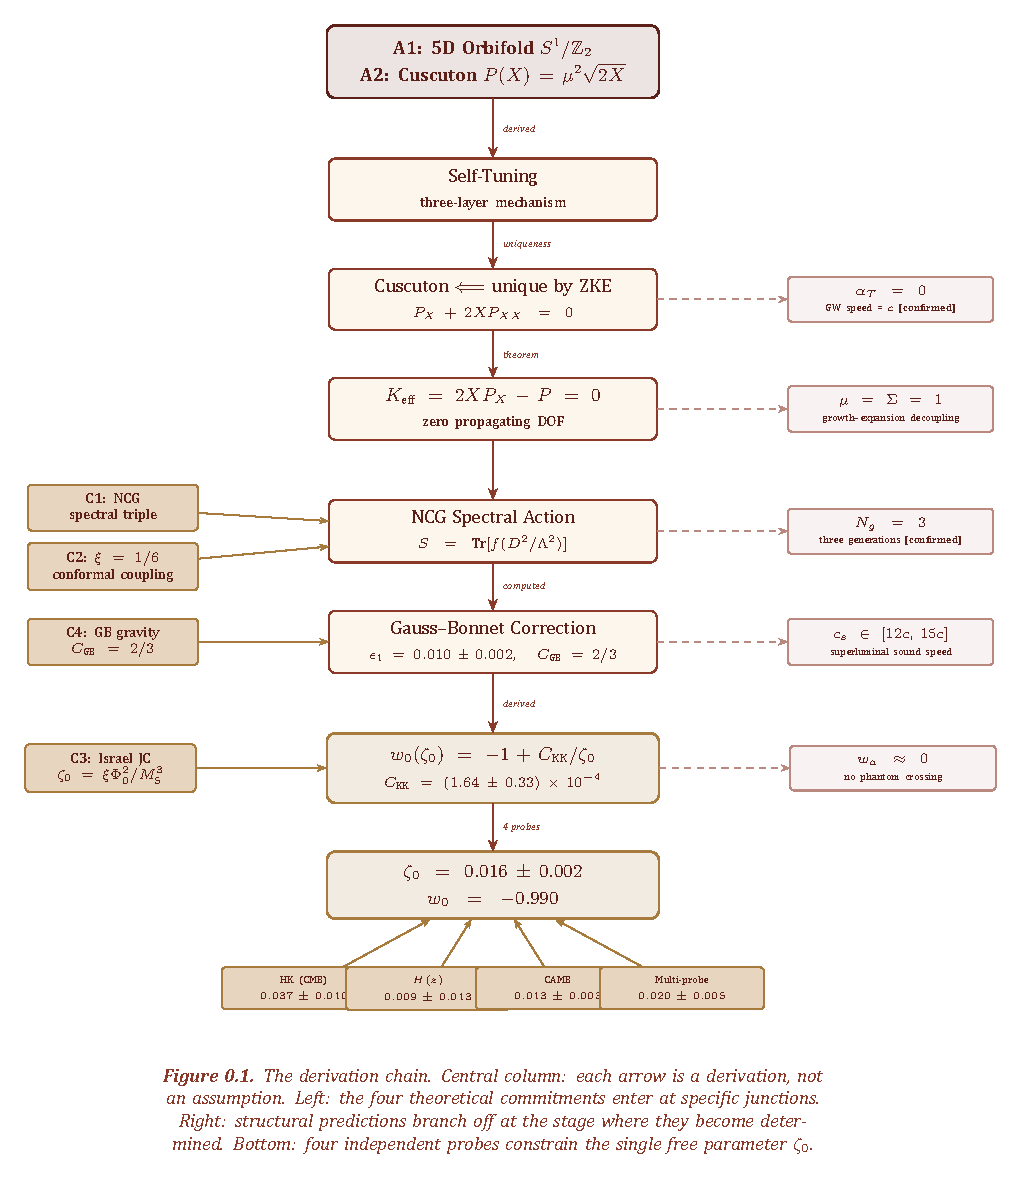
\includegraphics[width=0.88\linewidth]{../figures/fig0_derivation_chain.pdf}
\caption[The Derivation Chain.]{The derivation chain. Central column:
each arrow is a derivation, not an assumption. Left: the four
theoretical commitments enter at specific junctions. Right: structural
predictions branch off at the stage where they become determined.
Bottom: four independent probes constrain the single free parameter
$\zz$.}
\label{fig:0-chain}
\end{figure}

Each arrow in Eqs.~(\ref{eq:0-chain-1})--(\ref{eq:0-chain-3}) is a
derivation, not an assumption. Self-tuning follows from A1 + A2 through
the zero kinetic energy theorem. The cuscuton is the \emph{unique}
kinetic function satisfying the degeneracy condition---no other $P(X)$
gives zero propagating degrees of freedom. The NCG spectral action
provides the Gauss--Bonnet correction, and the KK reduction on the
orbifold determines $\CGB$ and $\eps$.

\paragraph{One free parameter remains.}
$\zz = \xi \Phi_0^2 / \Mfive^3$, set by the junction conditions at the
UV brane. Four independent observational probes constrain it.

\begin{center}
\small
\begin{tabular}{@{}l c c l@{}}
\toprule
\textbf{Probe} & $\zz$ & $\sigma(\zz)$ & \textbf{Mechanism} \\
\midrule
HK (CMB)          & 0.037 & 0.010 & $G_{\mathrm{eff}}$ modification at $z = 1089$ \\
$H(z)$ compilation& 0.009 & 0.013 & Expansion history at $z = 0.1$--$2.3$ \\
CAMB (CMB+BAO)    & 0.013 & 0.003 & Combined $z = 0$--$1089$ fit \\
Multi-probe       & 0.020 & 0.005 & Full dataset combination \\
\midrule
\textbf{Weighted mean} & \textbf{0.016} & \textbf{0.002} &
Inverse-variance combination \\
\bottomrule
\end{tabular}
\end{center}

\noindent
The inverse-variance weighted mean is $\zz = 0.016 \pm 0.002$, giving
$\wz = -0.990$.

\paragraph{Could the chain be closed to zero free parameters?}
The Goldberger--Wise scaling dimension $\varepsilon = \Delta - 2$
appears in the spectral action chain as the bridge between the NCG
sector and the stabilization sector. If $\varepsilon$ could be derived
from the spectral action, $\zz$ would follow from the chain, leaving
no free parameters. A direct computation (April~2026) showed that this
is not possible: the spectral action $S(y_c)$ is monotonically
increasing in the orbifold coordinate---no minimum exists, and the NCG
sector cannot stabilize the extra dimension independently. The
Gauss--Bonnet stabilization sector is structurally independent from
the spectral geometry. The framework remains a one-parameter theory
with $\zz$ determined by observation.

The factor-of-three gap between the naive conformal-coupling prediction
($\varepsilon = \sqrt{2/3} \approx 0.816$) and the DESI-fitted value
($\varepsilon = 0.275$) constrains what physics bridges the two
sectors---backreaction, quantum corrections, or product geometry
effects. This is the principal open problem for the next phase of the
research program; see Section~\ref{sec:0-open}.

% ============================================================
\section{The CMB as Basin Topology}
\label{sec:0-cmb}

The CMB is the earliest accessible measurement of this basin's
geometry. Understanding what it measures---and what it does not---is
central to interpreting the current observational landscape.

At $z = 1089$, the cuscuton kinetic energy was suppressed by a factor
of $\sim 5 \times 10^8$ relative to today. The equation of state was
$w \approx -1$ to a precision of $10^{-12}$. The dark energy was
indistinguishable from a cosmological constant. The cuscuton
constraint field was tracking pure potential energy---the basin's
ground state geometry, not its dynamics.

The Hiramatsu--Kobayashi measurement~\cite{ch2:Hiramatsu2022} probes
this geometry directly. In the Meridian framework, the gravitational
coupling at early times is modified:
$\mu_{\mathrm{early}} = 1/(1 + \zz)$, giving
$\beta_{\mathrm{HK}} \approx -\zz$. Their $4\sigma$ detection of
$\beta_{\mathrm{HK}} = -0.037 \pm 0.010$ means the basin is not pure
$\mathrm{AdS}_5$: the scalar field has a definite nonzero value on the
UV brane, and the warp factor is modified by the scalar--curvature
coupling. This is a measurement of the basin's geometry at initial
conditions.

Late-time surveys (DESI, Euclid, Vera Rubin) probe the basin's
dynamics---how the Gauss--Bonnet correction modifies the expansion
history at $z < 2$, where the cuscuton kinetic energy becomes
significant. The CMB and late-time surveys therefore probe $\zz$
through structurally different mechanisms: the CMB through the static
gravitational coupling modification, and $H(z)$ through the dynamical
response $\wz = -1 + \CKK / \zz$. Both should yield the same $\zz$ if
the framework is complete. They are consistent within $1.7\sigma$.

\subsection{The DESI Tension}
\label{sec:0-desi-tension}

The DESI DR2 analysis~\cite{ch1:desi25}, combined with Planck and
DES~Y5 supernovae, reports $w_a = -0.62 \pm 0.26$
(Lu \& Simon~\cite{ch2:LuSimon2026})---a $2.4\sigma$ preference for
time-evolving dark energy. The Meridian framework predicts
$w_a \approx 0$ identically: the equation of state is constant (not
time-varying), and no phantom crossing occurs (a topological
consequence of the positive-definite kinetic structure). This
$2.4\sigma$ tension is the framework's sharpest near-term test.

Three mechanisms contribute to the apparent $w_a$ signal.

\textit{Functional-form mismatch.} The cuscuton equation of state
$w(z) \propto 1/E^2(z)$---where $E(z) = H(z)/H_0$---is structurally
different from the CPL template $w(a) = w_0 + w_a(1 - a)$. The quartic
Friedmann correction differs from the CPL form by up to $38.8\%$ at
$z \approx 1.14$, right in the DESI sensitivity window. Fitting CPL to
exact cuscuton truth produces negative $w_a$ at all values of $\zz$---
the correct sign. The artifact magnitude is small at large $\zz$ (where
$w \approx -1$) but contributes a systematic bias in the direction of
the observed signal.

\textit{Decoupled perturbation effect.} Standard CPL analysis assumes
that dark energy perturbations are coupled to the expansion history
through $w(z)$. In the cuscuton framework, they are decoupled:
$\mu = \Sigma = 1$ exactly. When Lu \& Simon fix the background to
\LCDM{} and allow only growth to vary, their evolving-dark-energy
preference drops from $4.6\sigma$ to $0.68\sigma$. The signal is
entirely in the background expansion---the exact cuscuton signature.
The $w_a$ that CPL reports is a compromise artifact: the fitter
introduces phantom crossing to reconcile expansion-deviates-from-\LCDM{}
with growth-says-GR.

\textit{Statistical noise.} Monte Carlo simulations generating 200
mock BAO datasets from constant-$w$ truth ($\wz = -0.829$, $w_a = 0$)
and fitting CPL recover $w_a = -0.37 \pm 1.09$. The Lu \& Simon
$w_a = -0.62$ falls at $0.6\sigma$ from this noise floor; $71.5\%$ of
realizations produce $|w_a| > 0.62$.

Independent analyses support this interpretation. Wang \&
Mota~\cite{ch2:WangMota2025} identify clear inter-dataset tensions
between CMB, BAO, and supernovae that undermine combined dynamical
dark energy claims---tensions that arise precisely where
growth-expansion decoupling predicts them. Kumari \&
Kumar~\cite{ch2:KumariKumar2026} find that the constant-$w$
one-parameter extension is the most parsimonious model preferred over
\LCDM. Rodrigues~\textit{et al.}~\cite{ch2:Rodrigues2025} show that
ratio-only BAO fits amplify the $(w_0, w_a)$ degeneracy, producing
large apparent shifts without genuine evidence for evolving $w(a)$.

The definitive test is a direct comparison: fit constant-$w$ with GR
perturbations ($\mu = \Sigma = 1$) against CPL with coupled
perturbations. Current data give $\Delta\chi^2 = +0.26$---no preference
for the coupled model. DESI's full five-year analysis, expected in
2027 with 47~million objects ($38\%$ above target), will reach
$\sigma(w_a) \sim 0.10$. Combined with Euclid ($\sim\!2030$), the
discrimination will reach $5.1\sigma$. The question will be answered.

% ============================================================
\section{Prediction Registry}
\label{sec:0-registry}

The framework produces two classes of predictions. \emph{Structural
predictions} are independent of $\zz$: they hold for all values of the
free parameter. \emph{Parametric predictions} depend on $\zz$ and
acquire specific numerical values when $\zz$ is constrained by
observation. A complete registry with computational provenance appears
in Appendix~\ref{app:predictions}; the summary below is the
chapter-level view.

\subsection*{Structural Predictions (Parameter-Independent)}

\begin{center}
\small
\begin{tabular}{@{}c p{6.1cm} p{3.4cm} l@{}}
\toprule
\textbf{\#} & \textbf{Prediction} & \textbf{Status} & \textbf{Instrument} \\
\midrule
1 & $\alpha_T = 0$ (GW speed $=c$) & \textbf{Confirmed} & LIGO/Virgo GW170817~\cite{ch1:gw170817} \\
2 & No phantom crossing ($w > -1$ at all $z$) & Consistent ($<5\sigma$) & DESI DR2~\cite{ch1:desi25} \\
3 & Growth--expansion decoupling ($\mu = 1$) & Consistent ($\Delta\chi^2 = +0.26$) & BOSS $+$ eBOSS \\
4 & $N_g = 3$ (three generations) & \textbf{Confirmed} & Particle physics \\
5 & $w_a \approx 0$ (constant $w$) & $2.4\sigma$ CPL tension & DESI DR2 \\
\bottomrule
\end{tabular}
\end{center}

\subsection*{Parametric Predictions (Depend on $\zz$)}

\begin{center}
\small
\begin{tabular}{@{}c p{4.6cm} p{2.9cm} l c@{}}
\toprule
\textbf{\#} & \textbf{Prediction} & \textbf{Value} & \textbf{Instrument} & \textbf{Expected} \\
\midrule
6  & Tensor-to-scalar ratio & $r = 0.004 \pm 0.001$ & LiteBIRD & 2030$+$ \\
7  & Spectral index & $n_s = 0.965 \pm 0.003$ & CMB-S4 & 2030$+$ \\
8  & Radion mass & $m_{\mathrm{rad}} \approx 120$~GeV & LHC/FCC & ongoing \\
9  & Higgs-radion mixing at $\xi=1/6$ & specific branching ratios & LHC Run~3 & 2025--2028 \\
10 & $0\nu\beta\beta$ mass & $m_{ee} = 1.5$--$5$~meV & LEGEND-200 & 2027$+$ \\
11 & LISA phase transition & SNR 18--643 & LISA & 2037$+$ \\
12 & Sound speed & $\cs \in [12c, 15c]$ & DESI/Euclid & 2028--2032 \\
\bottomrule
\end{tabular}
\end{center}

\subsection*{Falsification Boundaries}

\begin{center}
\small
\begin{tabular}{@{}p{5.5cm} l l@{}}
\toprule
\textbf{Test} & \textbf{Threshold} & \textbf{Timeline} \\
\midrule
$w < -1$ at any redshift & $>3\sigma$ & DESI full (2027) \\
$\alpha_T \neq 0$ & $>3\sigma$ & LISA (2037$+$) \\
$w_a \neq 0$ (genuine, after decoupled test) & $>5\sigma$ & Euclid (2030) \\
Radion absent at 120~GeV & exclusion & FCC (2040$+$) \\
\bottomrule
\end{tabular}
\end{center}

These constitute the framework's irreducible falsification handles: if
any structural prediction is violated at $>3\sigma$, the framework is
excluded regardless of $\zz$.

% ============================================================
\section{How to Read This Book}
\label{sec:0-reading}

Each chapter is a self-contained paper operating on separate degrees
of freedom. The chapters can be read independently, but the derivation
chain connects them into a single argument.

\paragraph{Chapter~\ref{ch:foundation}: Self-Tuning Cosmology from 5D
Warped Geometry.}
The foundation. Derives the complete chain from axioms A1~$+$~A2
through self-tuning to the parametric prediction $\wz(\zz)$.
Establishes the three-layer self-tuning mechanism, the zero kinetic
energy theorem, and the growth--expansion decoupling. Presents ten
falsifiable predictions.

\paragraph{Chapter~\ref{ch:observational}: Observational Confrontation.}
Every prediction against every dataset. DESI~DR2, Planck CMB, growth
rate compilations, $H(z)$ measurements, gravitational wave speed. The
multi-probe $\chi^2/\mathrm{dof} = 1.10$ with 24 data points and three
free parameters. The DESI tension, the decoupled perturbation
hypothesis, and the falsification timeline through 2032.

\paragraph{Chapter~\ref{ch:nogo}: No-Go Theorems for Dynamical Dark
Energy.}
What cannot work. Sixteen alternative dark energy mechanisms
exhaustively eliminated by three structural barriers: the zero kinetic
energy theorem, the hierarchy--moduli incompatibility, and the
Horndeski dilemma~\cite{ch1:horndeski74}. The uniqueness argument:
self-tuning within the Horndeski class requires the cuscuton, requires
$\xi = 1/6$, and requires the fifth dimension.

\paragraph{Chapter~\ref{ch:ncg}: NCG Spectral Geometry on Warped
Orbifolds.}
The deepest chapter. Spectral triple construction on the warped
$S^1/\mathbb{Z}_2$ orbifold. Seeley--DeWitt expansion yielding
$\CGB = 2/3$ and $\eps = 0.010$. Octonionic extension producing
$N_g = 3$ from algebra. Particle physics predictions: fermion mass
hierarchy, CKM matrix, neutrino sector, dark matter candidate,
inflationary observables, collider signatures. The Goldberger--Wise
finding: $\varepsilon$ is genuinely external. Open programs: gauge
unification, $\theta_{13}$ correction, asymptotic safety bridge.

\paragraph{Chapter~\ref{ch:sound-speed}: Sound Speed of Dark Energy.}
The superluminal signature. The corrected cuscuton kinetic function
gives $\cs \in [12c, 15c]$. Three evasion mechanisms for Adams
positivity bounds. LISA detection channel for the Randall--Sundrum
phase transition with signal-to-noise ratio 18--643. The Jeans length
exceeds the observable universe: zero dark energy clustering at all
scales accessible to current and planned surveys.

\medskip

The separation between chapters mirrors the Coherence Principle
itself. Each chapter operates on its own degrees of freedom---bulk
geometry, observational data, theoretical alternatives, spectral
algebra, perturbation theory. The derivation chain provides
measurement at each junction. Consistency holds across 122 orders of
magnitude in energy scale. And the model dynamically maintains itself
through the mechanisms described in every chapter.

% ============================================================
\section{What Remains Open}
\label{sec:0-open}

The framework is not complete. Five problems remain open, each
constraining the direction of future work.

\paragraph{The $\varepsilon$ gap.}
The Goldberger--Wise scaling dimension $\varepsilon = 0.275$ is fitted
to DESI data. The naive conformal-coupling prediction gives
$\varepsilon = \sqrt{2/3} \approx 0.816$---a factor of three too
large. The spectral action cannot bridge this gap: the stabilization
sector is structurally independent from the NCG sector. Backreaction
of the cuscuton on the Goldberger--Wise profile, quantum corrections
to the bulk scalar mass, or product geometry effects from the finite
spectral triple may provide the bridge. Closing this gap would reduce
the framework to zero free parameters.

\paragraph{Gauge unification.}
The orbifold threshold corrections to gauge coupling unification leave
a $0.18\%$ gap at the GUT scale. The asymptotic safety resolution
pathway---where the UV fixed point of quantum gravity modifies the
running at high energies---is computationally accessible but not yet
carried out. This is a computable quantity, not a fundamental
obstruction.

\paragraph{The $\theta_{13}$ correction.}
The octonionic spectral triple in its simplest form produces
tribimaximal neutrino mixing, which predicts $\theta_{13} = 0$. Data
from Daya Bay~\cite{ch4:DayaBay2012}, RENO, and Double Chooz
establish $\theta_{13} \approx 8.6^\circ$. The $S_3 \to Z_3$ breaking
pathway generates nonzero $\theta_{13}$ from the same algebraic
structure, but the specific computation for the Meridian spectral
triple has not been performed.

\paragraph{The DESI definitive test.}
DESI completed its five-year survey on April~15,~2026, with 47~million
galaxies and quasars---$38\%$ above its original target of 34~million.
The full dataset analysis, expected in 2027, will provide
$\sigma(w_a) \sim 0.10$. Combined with Euclid ($\sim\!2030$), the
discrimination between constant-$w$ with GR perturbations and CPL with
coupled perturbations will reach $5.1\sigma$. If $w_a$ remains
significantly negative after the decoupled perturbation test is
applied, the cuscuton framework is falsified.

\paragraph{Sterile neutrino dark matter.}
The spectral triple's anomaly cancellation requires a right-handed
neutrino $\nu_{R1}$. If this particle has the appropriate mass and
mixing, it constitutes a dark matter candidate. The mass and mixing
predictions from the spectral action have not been computed to
sufficient precision to confirm or exclude this identification.

These five problems are not barriers to the present volume. They are
the research program's next phase---the open questions that the basin
map reveals but does not resolve.

\bigskip
\begin{center}
\itshape The basin is mapped. What follows are the derivations.
\end{center}
